\section{Stokes' Theorem}\label{sec:stokes}

So far the only types of line integrals which we have discussed are those along curves in $\mathbb{R}^{2}$. But the definitions and properties which were covered in Sections \ref{sec:line_int} and \ref{sec:line_int_props} can easily be extended to include functions of three variables, so that we can now discuss line integrals along curves in $\mathbb{R}^{3}$.

\definition{defn:lineintscalar3}{Scalar Line Integral}{For a real-valued function $f(x,y,z)$ and a curve $C$ in $\mathbb{R}^{3}$, parametrized by $x=x(t)$, $y=y(t)$, $z=z(t)$, $a \le t \le b$, the \textbf{line integral of} $f(x,y,z)$ \textbf{along} $C$ \textbf{with respect to arc length} $s$ is
 \[
  \int_C f(x,y,z)\,ds = \int_a^b f(x(t),y(t),z(t)) \,\sqrt{x\primeskip'(t)^2 + y\primeskip'(t)^2 + z\primeskip'(t)^2}\,\,dt .
 \]
 The \textbf{line integral of} $f(x,y,z)$ \textbf{along} $C$ \textbf{with respect to} $x$ is
 \[
  \int_C f(x,y,z)\,dx = \int_a^b f(x(t),y(t),z(t)) \,x\primeskip'(t)\,dt .
 \]
 The \textbf{line integral of} $f(x,y,z)$ \textbf{along} $C$ \textbf{with respect to} $y$ is
 \[
  \int_C f(x,y,z)\,dy = \int_a^b f(x(t),y(t),z(t)) \,y\primeskip'(t)\,dt .
 \]
 The \textbf{line integral of} $f(x,y,z)$ \textbf{along} $C$ \textbf{with respect to} $z$ is
 \[
  \int_C f(x,y,z)\,dz = \int_a^b f(x(t),y(t),z(t)) \,z\primeskip'(t)\,dt .
 \]}

Similar to the two-variable case, if $f(x,y,z) \ge 0$ then the line integral $\int_C f(x,y,z)\,ds$ can be thought of as the total area of the ``picket fence'' of height $f(x,y,z)$ at each point along the curve $C$ in $\mathbb{R}^{3}$.

Vector fields in $\mathbb{R}^{3}$ are defined in a similar fashion to those in $\mathbb{R}^{2}$, which allows us to define the line integral of a vector field along a curve in $\mathbb{R}^{3}$.

\definition{defn:lineintvec3}{Vector Line Integral}{For a vector field $\vecf(x,y,z) = P(x,y,z)\,\veci + Q(x,y,z)\,\vecj + R(x,y,z)\,\veck$ and a curve $C$ in $\mathbb{R}^{3}$ with a smooth parametrization $x=x(t)$, $y=y(t)$, $z=z(t)$, $a \le t \le b$, the \textbf{line integral of f along} $C$ is
 \begin{align*}
  \int_C \Dotprod{\vecf}{d\vecr} &= \int_C P(x,y,z)\,dx + \int_C Q(x,y,z)\,dy + \int_C R(x,y,z)\,dz\\
   &= \int_a^b \Dotprod{\vecf(x(t),y(t),z(t))}{\vecr\primeskip'(t)}\,dt ,
 \end{align*}
 where $\vecr(t)= x(t)\,\veci + y(t)\,\vecj + z(t)\,\veck$ is the position vector for points on $C$.}

Similar to the two-variable case, if $\vecf(x,y,z)$ represents the force applied to an object at a point $(x,y,z)$ then the line integral $\int_{C}{f}\cdot d\vec{r}$ represents the work done by that force in moving the object along the curve $C$ in $\mathbb{R}^{3}$.\index{work}

Some of the most important results we will need for line integrals in $\mathbb{R}^{3}$ are stated below without proof (the proofs are similar to their two-variable equivalents).

\begin{theorem}[Vector Line Integral Along a Curve]\label{thm:lineinttangent3}
For a vector field $\vecf(x,y,z) = P(x,y,z)\,\veci + Q(x,y,z)\,\vecj + R(x,y,z)\,\veck$ and a curve $C$ with a smooth parametrization $x=x(t)$, $y=y(t)$, $z=z(t)$, $a \le t \le b$ and position vector $\vecr(t) = x(t)\,\veci + y(t)\,\vecj + z(t)\,\veck$,
 \[
  \int_C \Dotprod{\vecf}{d\vecr} = \int_C \Dotprod{\vecf}{\vecT}\,ds ,
 \]
 where $\vecT(t) = \frac{\vecr\primeskip'(t)}{\norm{\vecr\primeskip'(t)}}$ is the unit tangent vector to $C$ at $(x(t),y(t),z(t))$.
\end{theorem}

% use thm:multi_chain2 instead

%\begin{theorem}[Chain Rule]\label{thm:chainrule3}
%If $w=f(x,y,z)$ is a continuously differentiable function of $x$, $y$, and $z$, and $x=x(t)$, $y=y(t)$ and $z=z(t)$ are differentiable functions of $t$, then $w$ is a differentiable function of $t$, and
% \[
%  \frac{dw}{dt} = \frac{\partial w}{\partial x}\,\frac{dx}{dt} + \frac{\partial w}{\partial y}\,\frac{dy}{dt} +
%   \frac{\partial w}{\partial z}\,\frac{dz}{dt} .
% \]
% Also, if $x=x(t_1,t_2)$, $y=y(t_1,t_2)$ and $z=z(t_1,t_2)$ are continuously differentiable function of $(t_1,t_2)$, then
% \[
%  \frac{\partial w}{\partial t_1} = \frac{\partial w}{\partial x}\,\frac{\partial x}{\partial t_1} +
%  \frac{\partial w}{\partial y}\,\frac{\partial y}{\partial t_1} +
%  \frac{\partial w}{\partial z}\,\frac{\partial z}{\partial t_1}
% \]
% and
% \[
%  \frac{\partial w}{\partial t_2} = \frac{\partial w}{\partial x}\,\frac{\partial x}{\partial t_2} +
%  \frac{\partial w}{\partial y}\,\frac{\partial y}{\partial t_2} +
%  \frac{\partial w}{\partial z}\,\frac{\partial z}{\partial t_2} .
% \]
%\end{theorem}
% % (See \cite[\S\,6.5]{tm} for a proof.)

\theorem{thm:lineintsuffpath3}{Fundamental Theorem of Line Integrals in Three Dimensions}{Let $\vecf(x,y,z) = P(x,y,z)\,\veci + Q(x,y,z)\,\vecj + R(x,y,z)\,\veck$ be a vector field in some solid $S$, with $P$, $Q$ and $R$ continuously differentiable functions on $S$. Let $C$ be a smooth curve in $S$ parametrized by $x=x(t)$, $y=y(t)$, $z=z(t)$, $a \le t \le b$. Suppose that there is a real-valued function $F(x,y,z)$ such that $\nabla F = \vecf$ on $S$. Then
 \begin{equation}\label{eqn:lineintsuffpath3}
  \int_C\vecf\cdot d\vec{r} = F(B) - F(A) ,
 \end{equation}
 where $A=(x(a),y(a),z(a))$ and $B=(x(b),y(b),z(b))$ are the endpoints of $C$.}

\theorem{cor:lineintsuffpath3}{Zero Line Integral}{If a vector field $\vecf$ has a potential in a solid $S$ without holes, then $\ds\oint_C\vecf\cdot d\vec{r} = 0$ for any closed curve $C$ in $S$ (i.e., $\ds\oint_{C}\Dotprod{\nabla F}{d\vecr} = 0$ for any real-valued function $F(x,y,z)$).}

\youtubeVideo{xVhHow_usMQ}{Fundamental Theorem for Line Integrals}

\mtable{Conical helix $C$ for \autoref{exmp_conhelix}.}{fig:conhelix}{%
\myincludeasythree{width=\marginparwidth,
3Droll=0.,
3Dortho=0.,
3Dc2c=0.52 -0.80 0.30,
3Dcoo=26.24 100.81 52.61,
3Droo=150.0}{width=\marginparwidth}{figures/conicalhelix}}

\example{exmp_conhelix}{Evaluating a Line Integral}{Let $f(x,y,z) = z$ and let $C$ be the curve in $\mathbb{R}^{3}$ parametrized by
\[x=t\sin t ,\quad y=t\cos t ,\quad z=t ,\quad 0\le t \le 8\pi .\]
Evaluate $\int_C f(x,y,z)\,ds$. (Note: $C$ is called a \emph{conical helix}\index{conical helix}\index{helix}. See \autoref{fig:conhelix}).}{Since $x\primeskip'(t)=\sin t + t\cos t$, $y\primeskip'(t)=\cos t - t\sin t$, and $z\primeskip'(t)=1$, we have
 \begin{align*}
  x\primeskip'(t)^2 + y\primeskip'(t)^2 + z\primeskip'(t)^2
   &= (\sin^2 t + 2t\sin t \cos t + t^2 \cos^2 t) \\
   & \qquad {} + (\cos^2 t - 2t\sin t \cos t + t^2 \sin^2 t) + 1\\
   &= t^2 (\sin^2 t + \cos^2 t) + \sin^2 t + \cos^2 t + 1\\
   &= t^2 + 2 ,
 \end{align*}
 so since $f(x(t),y(t),z(t)) = z(t) = t$ along the curve $C$, then
 \begin{align*}
  \int_C f(x,y,z)\,ds
   &= \int_0^{8\pi} f(x(t),y(t),z(t)) \,\sqrt{x\primeskip'(t)^2 + y\primeskip'(t)^2 + z\primeskip'(t)^2}\,\,dt\\
   &= \int_0^{8\pi} t\,\sqrt{t^2 + 2}\,\,dt\\
   &= \left.\left( \frac{1}{3} (t^2 + 2)^{3/2} \right) \,\right|_0^{8\pi}
   = \frac{1}{3} \left( (64\pi^2 + 2)^{3/2} - 2\sqrt{2} \right) .
 \end{align*}}

\example{exmp_conhelix2}{Evaluating a Line Integral}{Let $\vecf(x,y,z) = x\,\veci + y\,\vecj + 2z\,\veck$ be a vector field in $\mathbb{R}^{3}$. Using the same curve $C$ from \autoref{exmp_conhelix}, evaluate $\int_{C}{f}\cdot d\vec{r}$.}{It is easy to see that $F(x,y,z)=\frac{x^2}{2}+\frac{y^2}{2}+z^2$ is a potential for $\vecf(x,y,z)$ (i.e., $\nabla F = \vecf$). So by \autoref{thm:lineintsuffpath3} we know that
 \begin{align*}
  \int_C\vecf\cdot d\vec{r} &= F(B) - F(A) ,\text{ where $A=(x(0),y(0),z(0))$ and $B=(x(8\pi),y(8\pi),z(8\pi))$, so}\\
   &= F(8\pi\sin 8\pi,8\pi\cos 8\pi,8\pi) - F(0\sin 0,0\cos 0,0)\\
   &= F(0,8\pi,8\pi) - F(0,0,0)\\
   &= 0+\frac{(8\pi)^2}{2} + (8\pi)^2 - (0+0+0)
   = 96\pi^2 .
 \end{align*}}

We will now discuss a generalization of Green's Theorem in $\mathbb{R}^{2}$ to \emph{orientable} surfaces in $\mathbb{R}^{3}$, called \emph{Stokes' Theorem}.\index{Stokes' Theorem}\index{orientable}\index{surface!orientable} A surface $\Sigma$ in $\mathbb{R}^{3}$ is \textbf{orientable} if there is a continuous vector field \vecn\ in $\mathbb{R}^{3}$ such that \vecn\ is nonzero and normal to $\Sigma$ (i.e. perpendicular to the tangent plane) at each point of $\Sigma$. We say that such an \vecn\ is a \emph{normal vector field}.\index{normal vector field}\index{vector field!normal}

\mtable{An orientation of the sphere.}{fig:or_sph}{\begin{tikzpicture}
% todo Tim convert to asy
 \shade [ball color={\coloronefill!60!\colorone}] (0,0) circle (1.5);
 \draw [->] (0,0)--node[pos=1,above]{\small$y$} (2,0);
 \draw [->] (0,0)--node[pos=1,right]{\small$z$} (0,2);
 \draw [->] (0,0)--node[pos=1,right]{\small$x$} (0,0,4);
 \node[below]at(0,0){\small$0$};
 \draw [draw={\colorone}] (-1.5,0) arc (180:360:1.5 and 0.4);
 \draw [dashed,draw={\colorone}] (1.5,0) arc (0:180:1.5 and 0.4);
 \fill (0.98,0.98) circle (2pt);
 \draw [very thick,->] (0.98,0.98) -- (1.5,1.5)node[right]{\small $\vecn$};
 \draw [dashed,very thick,->] (0.98,0.98) -- (0.46,0.46)node[above left]{\small $-\vecn$};
\end{tikzpicture}}

For example, the unit sphere $x^2 + y^2 + z^2 = 1$ is orientable, since the continuous vector field $\vecn(x,y,z) = x\,\veci + y\,\vecj + z\,\veck$ is nonzero and normal to the sphere at each point. In fact, $-\vecn(x,y,z)$ is another normal vector field (see \autoref{fig:or_sph}). We see in this case that $\vecn(x,y,z)$ is what we have called an outward normal vector, and $-\vecn(x,y,z)$ is an \emph{inward} normal vector. These ``outward'' and ``inward'' normal vector fields on the sphere correspond to an ``outer'' and ``inner'' side, respectively, of the sphere. That is, we say that the sphere is a \emph{two-sided} surface.\index{surface!two-sided} Roughly, ``two-sided'' means ``orientable''. Other examples of two-sided, and hence orientable, surfaces are cylinders, paraboloids, ellipsoids, and planes.

You may be wondering what kind of surface would \emph{not} have two sides. An example is the \textbf{M\"{o}bius strip},\index{moebius@M\"{o}bius strip} which is constructed by taking a thin rectangle and connecting its ends at the opposite corners, resulting in a ``twisted'' strip (see \autoref{fig:mobius}).

\noindent\begin{minipage}[t]{\linewidth}\noindent%
\captionsetup{type=figure}%
 \flushinner{%
 \begin{tabular}{ccc}
  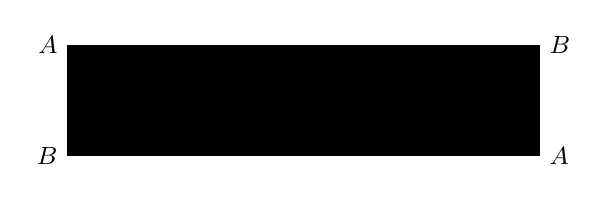
\begin{tikzpicture}
   \usetikzlibrary{arrows}
   \filldraw [draw={\colorone},fill={\coloronefill}]
    (0,  0)node[ left]{\small$B$} -- (6,  0)node[right]{\small$A$}
    --node[pos=.5,rotate=-90]{$\blacktriangleleft$}
    (6,1.4)node[right]{\small$B$} -- (0,1.4)node[ left]{\small$A$}
    --node[pos=.5,rotate= 90]{$\blacktriangleleft$} cycle;
  \end{tikzpicture}
 & \raisebox{.5in}{$\longrightarrow$} &
  \begin{tikzpicture}
   \usetikzlibrary{arrows}
   \filldraw [thick,draw={\colorone},fill={\coloronefill!50}] (0,1.4)
    -- (0,0) to[controls=+(90:1.5) and +(90:1.5)] (6,0)
    -- (6,1.4) to[controls=+(90:1.5) and +(90:1.5)] (0,1.4);
   \draw [dashed,draw={\colorone}] (0,0.7) to[out=-30,in=210,looseness=0.68]
    (6,0.7) to[controls=+(90:1.5) and +(90:1.5)] (0,0.7);
   \filldraw [fill opacity=0.3,draw={\colorone},thick,fill={\coloronefill}] (0,0)
    -- (0,1.4) to[out=-60,in=200,looseness=0.5] (6,0)
    -- (6,1.4) to[out=240,in=-20,looseness=0.5] (0,0);
   \node [scale=.13] at (3,2.2) {\psBill};
   \node at (3.5,2.2) {$\rightarrow$};
   \node [rotate=-180,cm={-1,0,0,1,(0,0)},scale=.13] at (2.4,1.5) {\psBill};
   \node at (1.9,1.4) {$\rightarrow$};
  \end{tikzpicture} \\
 Connect $A$ to $A$ and $B$ to $B$ along the ends & & Not orientable
 \end{tabular}}
 \caption{M\"{o}bius strip}
 \label{fig:mobius}
\end{minipage}

If you imagine walking along a line down the center of the M\"{o}bius strip, as in \autoref{fig:mobius}(b), then you arrive back at the same place from which you started but upside down! That is, your \emph{orientation} changed even though your motion was continuous along that center line. Informally, thinking of your vertical direction as a normal vector field along the strip, there is a discontinuity at your starting point (and, in fact, at every point) since your vertical direction takes two different values there. The M\"{o}bius strip has only \emph{one side}, and hence is nonorientable.% (For further discussion of orientability, see \cite[\S\,IV.7]{one}.)

For an orientable surface $\Sigma$ which has a boundary curve $C$, pick a unit normal vector \vecn\ such that if you walked along $C$ with your head pointing in the direction of \vecn, then the surface would be on your left. We say in this situation that \vecn\ is a \emph{positive unit normal vector}\index{vector!positive unit normal} and that $C$ is traversed \emph{\vecn-positively}\index{n-positive@\vecn-positive direction}. We can now state Stokes' Theorem:

\theorem{thm:stokes}{Stokes' Theorem}{\index{Stokes' Theorem}%
Let $\Sigma$ be an orientable surface in $\mathbb{R}^{3}$ whose boundary is a simple closed curve $C$, and let $\vecf(x,y,z) = P(x,y,z) \veci + Q(x,y,z) \vecj + R(x,y,z) \veck$ be a smooth vector field defined on some subset of $\mathbb{R}^{3}$ that contains $\Sigma$. Then
  \begin{equation}\label{eqn:stokes}
   \oint_C\vecf\cdot d\vec{r} = \iint_{\Sigma} \Dotprod{(\curl{\vecf}\,)}{\vecn}\,d\sigma ,
  \end{equation}
  where
  \begin{equation}\label{eqn:curl}
   \curl\vecf = \left( \frac{\partial R}{\partial y} - \frac{\partial Q}{\partial z} \right) \veci +
    \left( \frac{\partial P}{\partial z} - \frac{\partial R}{\partial x} \right) \vecj +
    \left( \frac{\partial Q}{\partial x} - \frac{\partial P}{\partial y} \right) \veck ,\index{curl}
  \end{equation}
  \vecn\ is a positive unit normal vector over $\Sigma$, and $C$ is traversed \vecn-positively.}

The formula for $\curl\vecf$ is unfortunately complicated.  If we recall that we have defined the operator $\nabla$ as a \emph{vector} in $\mathbb{R}^3$ by\index{$\nabla$}
\[
 \nabla = \frac{\partial}{\partial x}\,\veci + \frac{\partial}{\partial y}\,\vecj +
   \frac{\partial}{\partial z}\,\veck ,
\]
then we can write $\curl\vecf=\nabla\times\vecf$.

\begin{proof}
 As the general case is beyond the scope of this text, we will prove the theorem only for the special case where $\Sigma$ is the graph of $z=z(x,y)$ for some smooth real-valued function $z(x,y)$, with $(x,y)$ varying over a region $D$ in $\mathbb{R}^{2}$. \mtable{A particular case of Stokes' Theorem}{fig_stokes_eg}{\begin{tikzpicture}
%  \usetikzlibrary{arrows}
% todo Tim convert to asy
  \shade [ball color=\coloronefill] [rotate around={-20:(2.0,1.5)}] (2.0,1.5) ellipse (1.58 and 0.6);
  \draw [->] (0,0)--node[pos=1,above]{\small$y$} (4,0);
  \draw [->] (0,0)--node[pos=1,right]{\small$z$} (0,3);
  \draw [->] (0,0)--node[pos=1,right]{\small$x$} (0,0,3);
  \node[below]at(0,0){\small$0$};
  \filldraw [draw={\colorone},fill={\coloronefill}] (2,-0.7) ellipse (1.5 and 0.4);
  \draw [thick,->] (0.5,-0.7) arc (180:270:1.5 and 0.4);
  \draw [rotate around={-20:(2.0,1.5)}] (2.0,1.5) ellipse (1.58 and 0.6);
  \draw [rotate around={-20:(2.0,1.5)},thick,->] (0.42,1.5) arc (180:270:1.58 and 0.6);
  \fill (2.3,-0.85) circle (1pt);
  \fill (2.3,1.7) circle (1.2pt);
  \draw [very thick,->] (2.3,1.7) -- (2.7,2.3)node[right]{\small $\vecn$};
  \node [above] at (2.5,-0.83) {\small $(x,y)$};
  \node at (1.8,-0.6) {\small $D$};
  \node [below] at (2,-1.1) {\small $C_D$};
  \node [below] at (1.8,0.9) {\small $C$};
  \node [right] at (0.5,2.6) {\small $\Sigma: z = z(x,y)$};
  \draw [dashed] (0.5,-0.7) -- (0.5,1.7);
  \draw [dashed] (3.5,-0.7) -- (3.5,1);
 \end{tikzpicture}}
 Projecting $\Sigma$ onto the $xy$-plane, we see that the closed curve $C$ (the boundary curve of $\Sigma$) projects onto a closed curve $C_D$ which is the boundary curve of $D$ (see \autoref{fig_stokes_eg}). Assuming that $C$ has a smooth parametrization, its projection $C_D$ in the $xy$-plane also has a smooth parametrization, say
 \[C_D: x=x(t), y=y(t), a \le t \le b ,\]
 and so $C$ can be parametrized (in $\mathbb{R}^{3}$) as
 \[C: x=x(t), y=y(t), z=z(x(t),y(t)),a \le t \le b ,\]
 since the curve $C$ is part of the surface $z=z(x,y)$. Now, by the Chain Rule (\autoref{thm:multi_chain} in \autoref{sec:multi_chain}), for $z=z(x(t),y(t))$ as a function of $t$, we know that
 \[
  z\primeskip'(t) = \frac{\partial z}{\partial x}\,x\primeskip'(t) + \frac{\partial z}{\partial y}\,y\primeskip'(t) ,
 \]
 and so
 \begin{align*}
  \oint_C\vecf\cdot d\vec{r} &= \int_C P(x,y,z)\,dx + Q(x,y,z)\,dy + R(x,y,z)\,dz\\
   &= \int_a^b \left( P\,x\primeskip'(t) + Q\,y\primeskip'(t) +
    R\left( \frac{\partial z}{\partial x}\,x\primeskip'(t) + \frac{\partial z}{\partial y}\,y\primeskip'(t)
    \right) \right)\,dt\\
   &= \int_a^b \left( \left( P+R\,\frac{\partial z}{\partial x} \right) x\primeskip'(t) +
    \left( Q+R\,\frac{\partial z}{\partial y} \right) y\primeskip'(t) \right)\,dt\\
   &= \int_{C_D} \tilde{P}(x,y)\,dx + \tilde{Q}(x,y)\,dy ,
 \end{align*}
 where
 \begin{align*}
  \tilde{P}(x,y) &= P(x,y,z(x,y)) + R(x,y,z(x,y))\,\frac{\partial z}{\partial x}(x,y),\text{and}\\
  \tilde{Q}(x,y) &= Q(x,y,z(x,y)) + R(x,y,z(x,y))\,\frac{\partial z}{\partial y}(x,y)
 \end{align*}
 for $(x,y)$ in $D$. Thus, by Green's Theorem applied to the region $D$, we have
 \begin{equation}\label{eqn:stokesproof}
  \oint_C\vecf\cdot d\vec{r} = \iint_{D} \left( \frac{\partial \tilde{Q}}{\partial x} -
   \frac{\partial \tilde{P}}{\partial y} \right)\,dA .
 \end{equation}
 Thus,
 \begin{align*}
  \frac{\partial \tilde{Q}}{\partial x} &= \frac{\partial}{\partial x} \left( Q(x,y,z(x,y)) +
   R(x,y,z(x,y))\,\frac{\partial z}{\partial y}(x,y) \right) ,\text{ so by the Product Rule we get}\\
   &= \frac{\partial}{\partial x} \left( Q(x,y,z(x,y)) \right) + \left( \frac{\partial}{\partial x} R(x,y,z(x,y))
   \right) \frac{\partial z}{\partial y}(x,y) + R(x,y,z(x,y))\,\frac{\partial}{\partial x} \left(
   \frac{\partial z}{\partial y}(x,y) \right) .
 \end{align*}
 Now, by \autoref{thm:multi_chain2}, we have
 \begin{align*}
  \frac{\partial}{\partial x} \left( Q(x,y,z(x,y)) \right) &=
   \frac{\partial Q}{\partial x}\,\frac{\partial x}{\partial x} +
   \frac{\partial Q}{\partial y}\,\frac{\partial y}{\partial x} +
   \frac{\partial Q}{\partial z}\,\frac{\partial z}{\partial x}\\
   &= \frac{\partial Q}{\partial x} \cdot 1 + \frac{\partial Q}{\partial y} \cdot 0 + \frac{\partial Q}{\partial z}\,
    \frac{\partial z}{\partial x}\\
   &= \frac{\partial Q}{\partial x} + \frac{\partial Q}{\partial z}\,\frac{\partial z}{\partial x} .\\
  \intertext{Similarly,}
  \frac{\partial}{\partial x} \left( R(x,y,z(x,y)) \right) &=
   \frac{\partial R}{\partial x} + \frac{\partial R}{\partial z}\,\frac{\partial z}{\partial x} .
\end{align*}
 Thus,
 \begin{align*}
  \frac{\partial \tilde{Q}}{\partial x} &= \frac{\partial Q}{\partial x} + \frac{\partial Q}{\partial z}\,
   \frac{\partial z}{\partial x} + \left( \frac{\partial R}{\partial x} + \frac{\partial R}{\partial z}\,
   \frac{\partial z}{\partial x} \right) \frac{\partial z}{\partial y} + R(x,y,z(x,y))\,
   \frac{\partial^2 z}{\partial x \, \partial y}\\
   &= \frac{\partial Q}{\partial x} + \frac{\partial Q}{\partial z}\,\frac{\partial z}{\partial x} +
    \frac{\partial R}{\partial x}\,\frac{\partial z}{\partial y} + \frac{\partial R}{\partial z}\,
    \frac{\partial z}{\partial x}\,\frac{\partial z}{\partial y} + R\,\frac{\partial^2 z}{\partial x \, \partial y}.\\
  \intertext{In a similar fashion, we can calculate}
  \frac{\partial \tilde{P}}{\partial y} &= \frac{\partial P}{\partial y} +
   \frac{\partial P}{\partial z}\,\frac{\partial z}{\partial y} +
    \frac{\partial R}{\partial y}\,\frac{\partial z}{\partial x} + \frac{\partial R}{\partial z}\,
    \frac{\partial z}{\partial y}\,\frac{\partial z}{\partial x} + R\,\frac{\partial^2 z}{\partial y \, \partial x}.
 \end{align*}
 So subtracting gives
 \begin{equation}\label{eqn:stokeslong}
  \frac{\partial \tilde{Q}}{\partial x} - \frac{\partial \tilde{P}}{\partial y} =
   \left( \frac{\partial Q}{\partial z} - \frac{\partial R}{\partial y} \right) \frac{\partial z}{\partial x}
   + \left( \frac{\partial R}{\partial x} - \frac{\partial P}{\partial z}\right) \frac{\partial z}{\partial y}
   + \left( \frac{\partial Q}{\partial x} - \frac{\partial P}{\partial y} \right)
 \end{equation}
 since $\frac{\partial^2 z}{\partial x \, \partial y} = \frac{\partial^2 z}{\partial y \, \partial x}$ by the
 smoothness of $z=z(x,y)$. Hence, by \autoeqref{eqn:stokesproof},
 \begin{equation}\label{eqn:stokespart1}
  \oint_C\vecf\cdot d\vec{r} = \iint_{D} \left(
   -\left( \frac{\partial R}{\partial y} - \frac{\partial Q}{\partial z} \right) \frac{\partial z}{\partial x}
   -\left( \frac{\partial P}{\partial z} - \frac{\partial R}{\partial x} \right) \frac{\partial z}{\partial y}
   + \left( \frac{\partial Q}{\partial x} - \frac{\partial P}{\partial y} \right) \right)\,dA
 \end{equation}
 after factoring out a $-1$ from the terms in the first two products in \autoeqref{eqn:stokeslong}.
 
 Now, recall from \autoref{sec:multi_tangent} that the vector $\vecn = -\frac{\partial z}{\partial x}\,\veci - \frac{\partial z}{\partial y}\,\vecj + \veck$ is normal to the tangent plane to the surface $z=z(x,y)$ at each point of $\Sigma$. Thus,
 \[
  \vecn = \frac{\vecn}{\norm{\vecn}} =
   \frac{-\frac{\partial z}{\partial x}\,\veci - \frac{\partial z}{\partial y}\,\vecj +
   \veck}{\sqrt{1 + \left( \tfrac{\partial z}{\partial x} \right)^2 +
   \left( \tfrac{\partial z}{\partial y} \right)^2}}
 \]
 is in fact a positive unit normal vector to $\Sigma$ (see \autoref{fig_stokes_eg}). Hence, using the parametrization $\vecr(x,y) = x\,\veci + y\,\vecj + z(x,y)\,\veck$, for $(x,y)$ in $D$, of the surface $\Sigma$, we have $\frac{\partial \vecr}{\partial x} = \veci + \frac{\partial z}{\partial x}\,\veck$ and $\frac{\partial \vecr}{\partial y} = \vecj + \frac{\partial z}{\partial y}\,\veck$, and so $\norm{\frac{\partial \vecr}{\partial x}\times\frac{\partial \vecr}{\partial y}} = \sqrt{1 + \left( \tfrac{\partial z}{\partial x} \right)^2 + \left( \tfrac{\partial z}{\partial y} \right)^2}$. So we see that using \autoeqref{eqn:curl} for $\curl{\vecf}$, we have
 \begin{align*}
  \iint_{\Sigma} & \Dotprod{(\curl{\vecf})}{\vecn}\,d\sigma \\
  &=
   \iint_{D} \Dotprod{(\curl{\vecf}\,)}{\vecn}\,
   \norm{\frac{\partial \vecr}{\partial x}\times\frac{\partial \vecr}{\partial y}}\,dA\\
   &= \iint_{D} \Dotprod{\left( \left( \frac{\partial R}{\partial y} - \frac{\partial Q}{\partial z} \right)
    \veci + \left( \frac{\partial P}{\partial z} - \frac{\partial R}{\partial x} \right) \vecj +
    \left( \frac{\partial Q}{\partial x} - \frac{\partial P}{\partial y} \right) \veck
    \right)}{\left( -\frac{\partial z}{\partial x}\veci - \frac{\partial z}{\partial y}\vecj +
    \veck \right)} dA\\
   &= \iint_{D} \left(
    -\left( \frac{\partial R}{\partial y} - \frac{\partial Q}{\partial z} \right) \frac{\partial z}{\partial x}
    -\left( \frac{\partial P}{\partial z} - \frac{\partial R}{\partial x} \right) \frac{\partial z}{\partial y}
    + \left( \frac{\partial Q}{\partial x} - \frac{\partial P}{\partial y} \right) \right)\,dA ,
 \end{align*}
 which, upon comparing to \autoeqref{eqn:stokespart1}, proves the Theorem.
\end{proof}

Note: The condition in Stokes' Theorem that the surface $\Sigma$ have a (continuously varying) positive unit normal vector \vecn\ and a boundary curve $C$ traversed \vecn-positively can be expressed more precisely as follows: if $\vecr(t)$ is the position vector for $C$ and $\vecT(t) = \vecr\primeskip'(t)/\norm{\vecr\primeskip'(t)}$ is the unit tangent vector to $C$, then the vectors \vecT, \vecn, $\vecT\times\vecn$ form a right-handed system.

Also, it should be noted that Stokes' Theorem holds even when the boundary curve $C$ is piecewise smooth.

\example{exmp_stokesparab}{Verifying Stokes' Theorem}{Verify Stokes' Theorem for $\vecf(x,y,z) = z\,\veci + x\,\vecj + y\,\veck$ when $\Sigma$ is the paraboloid $z=x^2 + y^2$ such that $z \le 1$ (see \autoref{fig_parab_stokes}).%
 \mtable{$z=x^2 + y^2$ for \autoref{exmp_stokesparab}.}{fig_parab_stokes}{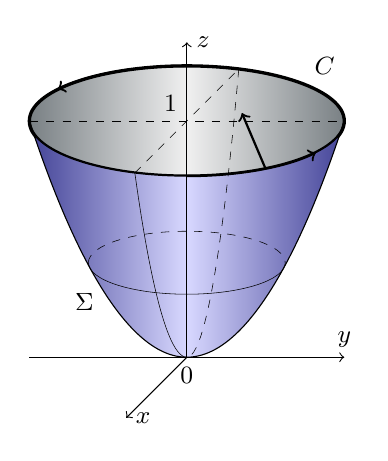
\begin{tikzpicture}
 % todo Tim convert to asy
  \usetikzlibrary{arrows}
  \definecolor{insideo}{HTML}{798084}
  \definecolor{insidei}{HTML}{F0F0F0}
  \definecolor{outer}{HTML}{424296}
  \definecolor{inner}{HTML}{D8D8FF}
  \shadedraw [left color=insideo,right color=insideo,middle color=insidei,line width=1.2pt] (0,3) ellipse (2 and 0.7);
  \shadedraw [left color=outer,right color=outer,middle color=inner]
  (2,3) arc (360:180:2 and 0.7) -- (-2,3) parabola bend (0,0) (2,3);
  \draw [dashed,line width=0.2pt] (-2,3) -- (2,3);
  \draw [dashed,line width=0.2pt] (-0.66,2.34) -- (0.66,3.66);
  \draw [line width=0.2pt] (-0.66,2.34) parabola [bend at end] (0,0);
  \draw [dashed,line width=0.2pt] (0.66,3.66) parabola [bend at end] (0,0);
  \draw [line width=0.2pt] (-1.25,1.2) arc (180:360:1.25 and 0.4);
  \draw [dashed,line width=0.2pt] (-1.25,1.2) arc (180:0:1.25 and 0.4);
  \draw [->] (-2,0)--node[pos=1,above]{\small$y$} (2,0);
  \draw [->] (0,0)--node[pos=1,right]{\small$z$} (0,4);
  \draw [->] (0,0)--node[pos=1,right]{\small$x$} (0,0,2);
  \draw [thick,->] (0,2.3) arc (270:325:2 and 0.7);
  \draw [thick,->] (0,3.7) arc (90:145:2 and 0.7);
  \draw [thick,->] (1,2.3938) -- (0.7,3.1)node[above]{\small $\vecn$};
  \node[below]at(0,0){\small$0$};
  \node [right] at (1.5,3.7) {\small $C$};
  \node at (-1.3,0.7) {\small $\Sigma$};
  \node [above left] at (0,3) {\small $1$};
 \end{tikzpicture}}%
 }{The positive unit normal vector to the surface $z=z(x,y)=x^2 + y^2$ is
 \[
  \vecn =
   \frac{-\frac{\partial z}{\partial x}\,\veci - \frac{\partial z}{\partial y}\,\vecj +
   \veck}{\sqrt{1 + \left( \tfrac{\partial z}{\partial x} \right)^2 +
   \left( \tfrac{\partial z}{\partial y} \right)^2}} =
   \frac{-2x\,\veci - 2y\,\vecj + \veck}{\sqrt{1 + 4x^2 + 4y^2}} ,
 \]
 and $\curl\vecf= (1-0)\,\veci+(1-0)\,\vecj+(1-0)\,\veck = \veci+\vecj+\veck$, so
 \[
  \Dotprod{(\curl{\vecf}\,)}{\vecn} = (-2x-2y+1)/\sqrt{1 + 4x^2 + 4y^2} .
 \]
 Since $\Sigma$ can be parametrized as $\vecr(x,y) = x\,\veci+y\,\vecj+(x^2 + y^2 )\,\veck$ for $(x,y)$ in the region $D = \lbrace \, (x,y):\,x^2 + y^2 \le 1 \,\rbrace$, then
 \begin{align*}
  \iint_{\Sigma} \Dotprod{(\curl{\vecf}\,)}{\vecn}\,d\sigma &=
   \iint_{D} \Dotprod{(\curl{\vecf}\,)}{\vecn}\,
   \norm{\frac{\partial \vecr}{\partial x}\times\frac{\partial \vecr}{\partial y}}\,dA\\
   &= \iint_{D} \frac{-2x-2y+1}{\sqrt{1 + 4x^2 + 4y^2}}\,\sqrt{1 + 4x^2 + 4y^2}\,dA\\
   &= \iint_{D} (-2x-2y+1)\,dA ,\text{ so switching to polar coordinates gives}\\
   &= \int_0^{2\pi} \int_0^1 (-2r\cos \theta - 2r\sin \theta + 1)r\,dr\,d\theta\\
   &= \int_0^{2\pi} \int_0^1 (-2r^2 \cos \theta - 2r^2 \sin \theta + r)\,dr\,d\theta\\
   &= \int_0^{2\pi} \left( -\tfrac{2r^3}{3} \cos \theta - \tfrac{2r^3}{3} \sin \theta +
   \tfrac{r^2}{2}\,\Big|_{r=0}^{r=1} \,\right)\,d\theta\\
   &= \int_0^{2\pi} \left( -\tfrac{2}{3} \cos \theta - \tfrac{2}{3} \sin \theta + \tfrac{1}{2} \right)\,d\theta\\
   &= \left.-\tfrac{2}{3} \sin \theta + \tfrac{2}{3} \cos \theta + \tfrac{1}{2}\theta\,\right|_0^{2\pi} = \pi .
 \end{align*}
 The boundary curve $C$ is the unit circle $x^2 + y^2 =1$ laying in the plane $z=1$ (see \autoref{fig_parab_stokes}), which can be parametrized as $x = \cos t$, $y = \sin t$, $z = 1$ for $0 \le t \le 2\pi$. So
 \begin{align*}
  \oint_C\vecf\cdot d\vec{r} &= \int_0^{2\pi} ((1)(-\sin t) + (\cos t)(\cos t) + (\sin t)(0))\,dt\\
   &= \int_0^{2\pi} \left( -\sin t + \frac{1+\cos 2t}{2} \right) \,dt \quad \left( \text{here we used $\cos^2 t =
   \frac{1+\cos 2t}{2}$} \right)\\
   &= \left.\cos t + \frac{t}{2} + \frac{\sin 2t}{4}\,\right|_0^{2\pi} = \pi .
 \end{align*}
 So we see that $\oint_C\vecf\cdot d\vec{r}=\iint_{\Sigma} \Dotprod{(\curl{\vecf}\,)}{\vecn} \,d\sigma$, as predicted by Stokes' Theorem.}

The line integral in the preceding example was far simpler to calculate than the surface integral, but this will not always be the case.

\example{ex_use_stokes}{Using Stokes' Theorem}{Let $\Sigma$ be the elliptic paraboloid $z=\frac{x^2}{4}+\frac{y^2}{9}$ for $z \le 1$, and let $C$ be its boundary curve. Calculate $\oint_C\vecf\cdot d\vec{r}$ for $\vecf(x,y,z)=(9xz+2y)\veci+(2x+y^2 )\vecj+(-2y^2 +2z)\veck$, where $C$ is traversed counterclockwise.}{The surface is similar to the one in \autoref{exmp_stokesparab}, except now the boundary curve $C$ is the ellipse $\frac{x^2}{4}+\frac{y^2}{9}=1$ laying in the plane $z=1$. In this case, using Stokes' Theorem is easier than computing the line integral directly. As in \autoref{exmp_stokesparab}, at each point $(x,y,z(x,y))$ on the surface $z=z(x,y)=\frac{x^2}{4}+\frac{y^2}{9}$ the vector
 \[
  \vecn =
   \frac{-\frac{\partial z}{\partial x}\,\veci - \frac{\partial z}{\partial y}\,\vecj +
   \veck}{\sqrt{1 + \left( \tfrac{\partial z}{\partial x} \right)^2 +
   \left( \tfrac{\partial z}{\partial y} \right)^2}} =
   \frac{-\tfrac{x}{2}\,\veci - \tfrac{2y}{9}\,\vecj + \veck}{\sqrt{1 +\tfrac{x^2}{4}+
    \tfrac{4y^2}{9}}} ,
 \]
 is a positive unit normal vector to $\Sigma$. And calculating the curl of \vecf\ gives
 \[
  \curl\vecf = (-4y-0)\veci + (9x-0)\vecj + (2-2)\veck = -4y\,\veci + 9x\,\vecj +
   0\,\veck,
 \]
 so
 \[
  \Dotprod{(\curl{\vecf}\,)}{\vecn} = \frac{(-4y)(-\tfrac{x}{2})+(9x)(-\tfrac{2y}{9})+
   (0)(1)}{\sqrt{1 +\tfrac{x^2}{4}+\tfrac{4y^2}{9}}} = \frac{2xy-2xy+0}{\sqrt{1 +\tfrac{x^2}{4}+\tfrac{4y^2}{9}}} = 0,
 \]
 and so by Stokes' Theorem
 \[
  \oint_C\vecf\cdot d\vec{r} = \iint_{\Sigma} \Dotprod{(\curl{\vecf}\,)}{\vecn}\,d\sigma =
   \iint_{\Sigma} 0\,d\sigma = 0 .
 \]}

In physical applications, for a simple closed curve $C$ the line integral $\oint_C\vecf\cdot d\vec{r}$ is often called the \textbf{circulation}\index{circulation} of \vecf\ around $C$. For example, if \vecE\ represents the electrostatic field due to a point charge, then it turns out
% (See Ch. 2 in \cite{rmc}.)
that $\curl\vecE = \vec0$, which means that the circulation $\oint_C\vecE\cdot d\vec{r}=0$ by Stokes' Theorem. Vector fields which have zero curl are often called \emph{irrotational}\index{irrotational} fields.

In fact, the term curl was created by the 19\textsuperscript{th} century Scottish physicist James Clerk Maxwell in his study of electromagnetism, where it is used extensively. In physics, the curl is interpreted as a measure of \emph{circulation density}. This is best seen by using another definition of curl \vecf\ which is equivalent
% (See \cite{sch}, p. 78-81, for the derivation.)
to the definition given by \autoeqref{eqn:curl}. Namely, for a point $(x,y,z)$ in $\mathbb{R}^{3}$,
\[
 \Dotprod{\vecn}{(\curl\vecf\,)}(x,y,z)
 = \lim_{S \to 0} \frac{1}{S} \oint_C\vecf\cdot d\vec{r} ,
\]
where $S$ is the surface area of a surface $\Sigma$ containing the point $(x,y,z)$ and with a simple closed boundary curve $C$ and positive unit normal vector \vecn at $(x,y,z)$. In the limit, think of the curve $C$ shrinking to the point $(x,y,z)$, which causes $\Sigma$, the surface it bounds, to have smaller and smaller surface area. That ratio of circulation to surface area in the limit is what makes the curl a rough measure of circulation density (i.e., circulation per unit area).

\noindent\begin{minipage}[t]{\linewidth}\noindent%
\captionsetup{type=figure}%
\centering
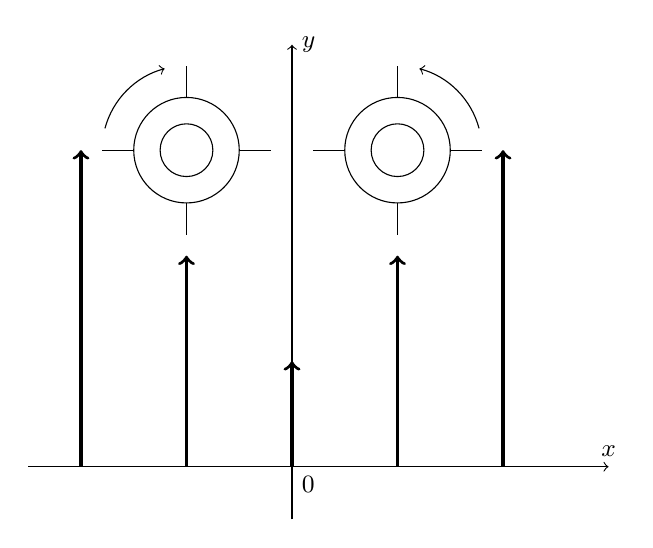
\begin{tikzpicture}[scale=1.34]
 \usetikzlibrary{arrows}
 \draw [->] (-2.5,0) -- (3,0)node[above]{\small$x$};
 \draw [->] (0,-0.5) -- (0,4)node[right]{\small$y$};
 \node[below right] at (0,0) {\small $0$};
 \draw [draw={\colorone},very thick,->] (-2,0) -- (-2,3);
 \draw [draw={\colorone},very thick,->] (-1,0) -- (-1,2);
 \draw [draw={\colorone},very thick,->] (0,0) -- (0,1);
 \draw [draw={\colorone},very thick,->] (1,0) -- (1,2);
 \draw [draw={\colorone},very thick,->] (2,0) -- (2,3) node[below right]{$\vecf$};
 \draw [draw={\colorone}] (1,3) circle (0.5) circle(0.25);
 \draw [draw={\colorone}] (1.5,3) -- (1.8,3);
 \draw [draw={\colorone}] (0.5,3) -- (0.2,3);
 \draw [draw={\colorone}] (1,3.5) -- (1,3.8);
 \draw [draw={\colorone}] (1,2.5) -- (1,2.2);
 \draw [draw={\colorone},->] (1,3) ++(15:0.8) arc (15:75:0.8);
 \draw [draw={\colorone}] (-1,3) circle (0.5) circle (0.25);
 \draw [draw={\colorone}] (-1.5,3) -- (-1.8,3);
 \draw [draw={\colorone}] (-0.5,3) -- (-0.2,3);
 \draw [draw={\colorone}] (-1,3.5) -- (-1,3.8);
 \draw [draw={\colorone}] (-1,2.5) -- (-1,2.2);
 \draw [draw={\colorone},->] (-1,3) ++(165:0.8) arc (165:105:0.8);
\end{tikzpicture}
\caption{Curl and rotation}\label{fig_curl_rot}
\end{minipage}

An idea of how the curl of a vector field is related to rotation is shown in \autoref{fig_curl_rot}. Suppose we have a vector field $\vecf(x,y,z)$ which is always parallel to the $xy$-plane at each point $(x,y,z)$ and that the vectors grow larger the further the point $(x,y,z)$ is from the $y$-axis. For example, $\vecf(x,y,z) = (1+x^2 )\,\vecj$. Think of the vector field as representing the flow of water, and imagine dropping two wheels with paddles into that water flow, as in \autoref{fig_curl_rot}. Since the flow is stronger (i.e., the magnitude of \vecf\ is larger) as you move away from the $y$-axis, then such a wheel would rotate counterclockwise if it were dropped to the right of the $y$-axis, and it would rotate clockwise if it were dropped to the left of the $y$-axis. In both cases the curl would be nonzero ($\curl\vecf(x,y,z) = 2x\,\veck$ in our example) and would obey the right-hand rule, that is, $\curl\vecf(x,y,z)$ points in the direction of your thumb as you cup your right hand in the direction of the rotation of the wheel. So the curl points outward (in the positive $z$-direction) if $x > 0$ and points inward (in the negative $z$-direction) if $x < 0$. Notice that if all the vectors had the same direction \emph{and} the same magnitude, then the wheels would not rotate and hence there would be no curl (which is why such fields are called irrotational, meaning no rotation).

Finally, by Stokes' Theorem, we know that if $C$ is a simple closed curve in some solid region $S$ in $\mathbb{R}^{3}$ and if $\vecf(x,y,z)$ is a smooth vector field such that $\curl\vecf = \vec0$ in $S$, then
\[
 \oint_C\vecf\cdot d\vec{r} = \iint_{\Sigma} \Dotprod{(\curl{\vecf}\,)}{\vecn}\,d\sigma =
   \iint_{\Sigma} \Dotprod{\vec0}{\vecn}\,d\sigma = \iint_{\Sigma} 0\,d\sigma = 0 ,
\]
where $\Sigma$ is any orientable surface inside $S$ whose boundary is $C$ (such a surface is sometimes called a \emph{capping surface} for $C$\index{capping surface}). So similar to the two-variable case, we have a three-dimensional version of a result from \autoref{sec:greens}, for solid regions in $\mathbb{R}^{3}$ which are \textbf{simply connected}\index{simply connected} (i.e. regions having no holes):\index{path independence}\index{exact differential form}

\theorem{thm:irrot_equiv}{Irrotational Equivalences}{The following statements are equivalent for a simply connected solid region $S$ in $\mathbb{R}^{3}$:
  \begin{enumerate}
  \item $\vecf(x,y,z) = P(x,y,z)\,\veci + Q(x,y,z)\,\vecj + R(x,y,z)\,\veck$ has a smooth potential $F(x,y,z)$ in $S$
  \item $\ds\int_C\vecf\cdot d\vec{r}$ is independent of the path for any curve $C$ in $S$
  \item $\ds\oint_C\vecf\cdot d\vec{r} = 0$ for every simple closed curve $C$ in $S$
  \item $\dfrac{\partial R}{\partial y} = \dfrac{\partial Q}{\partial z}$,   $\dfrac{\partial P}{\partial z} = \dfrac{\partial R}{\partial x}$, and   $\dfrac{\partial Q}{\partial x} = \dfrac{\partial P}{\partial y}$ in $S$ (i.e., $\curl\vecf = \vec0$ in $S$, or the differential form $P\,dx + Q\,dy + R\,dz$ is exact)
 \end{enumerate}}

\example{ex_check_irrot}{Determining Irrotation}{Determine if the vector field $\vecf(x,y,z) = xyz\,\veci + xz\,\vecj + xy\,\veck$ has a potential in $\mathbb{R}^{3}$.}{Since $\mathbb{R}^{3}$ is simply connected, we just need to check whether $\curl\vecf = \vec0$ throughout $\mathbb{R}^{3}$, that is,
 \[
  \frac{\partial R}{\partial y} = \frac{\partial Q}{\partial z},\quad
  \frac{\partial P}{\partial z} = \frac{\partial R}{\partial x},\quad\text{and}\quad
  \frac{\partial Q}{\partial x} = \frac{\partial P}{\partial y}
 \]
 throughout $\mathbb{R}^{3}$, where $P(x,y,z)=xyz$, $Q(x,y,z)=xz$, and $R(x,y,z)=xy$. But we see that
 \[
  \frac{\partial P}{\partial z} = xy , \frac{\partial R}{\partial x} = y \quad\Rightarrow\quad
  \frac{\partial P}{\partial z} \ne \frac{\partial R}{\partial x} \text{ for some $(x,y,z)$ in $\mathbb{R}^{3}$.}
 \]
 Thus, $\vecf(x,y,z)$ does not have a potential in $\mathbb{R}^{3}$.}

The theorems in this chapter all relate an integral over a domain to an integral over the boundary of the domain.  This means that we need to pay special attention to the orientation of the domain.  We'll occasionally use the symbol $\partial$ to indicate the boundary of something (so the boundary of $D$ would be $\partial D$).  This is the same symbol as a partial derivative, so you'll have to look at the context to figure out which definition is being used.

We also have four new theorems about these types of integrals. These are similar to the Fundamental Theorem of Calculus, so we'll put all five together into \autoref{fundThms}.

% todo Tim check the phrasing
{
\tcbset{grow to right by=100pt}
\keyidea{fundThms}{Fundamental Theorems Relating Integrals and Domains}{%
\renewcommand{\arraystretch}{1.4}
 \begin{tabular}{p{.25\specialboxlength} l p{.35\specialboxlength}}
  Theorem & Equation & Orientation \\\midrule
  Fundamental Theorem\par of Calculus & $f(b)-f(a)=\int_a^b \fp(x)d x$ &\\
  Fundamental Theorem\par of Gradient Fields & $\phi(Q)-\phi(P)=\int_C\nabla\phi\cdot d s$ & $C$ goes from $P$ to $Q$ \\
  Green's Theorem & $\oint_{\partial D}Pd x+Qdy=\iint_D Q_x-P_yd A$ & $\partial D$ oriented counterclockwise \\
  Stokes' Theorem & $\int_{\partial S}\vec F\cdot d\vec r=\iint_S\curl\vec F\cdot \vecn d\sigma$ & $\partial S$ oriented with $S$ to the left \\
  Divergence Theorem & $\iint_{\partial W}\vec F\cdot d \vec\sigma=\iiint_W\Div\vec Fd V$ & $\partial W$ oriented outwards
 \end{tabular}}
}

\printexercises{exercises/14_Stokes_exercises}
